% Options for packages loaded elsewhere
\PassOptionsToPackage{unicode}{hyperref}
\PassOptionsToPackage{hyphens}{url}
%
\documentclass[
]{article}
\usepackage{lmodern}
\usepackage{amssymb,amsmath}
\usepackage{ifxetex,ifluatex}
\ifnum 0\ifxetex 1\fi\ifluatex 1\fi=0 % if pdftex
  \usepackage[T1]{fontenc}
  \usepackage[utf8]{inputenc}
  \usepackage{textcomp} % provide euro and other symbols
\else % if luatex or xetex
  \usepackage{unicode-math}
  \defaultfontfeatures{Scale=MatchLowercase}
  \defaultfontfeatures[\rmfamily]{Ligatures=TeX,Scale=1}
\fi
% Use upquote if available, for straight quotes in verbatim environments
\IfFileExists{upquote.sty}{\usepackage{upquote}}{}
\IfFileExists{microtype.sty}{% use microtype if available
  \usepackage[]{microtype}
  \UseMicrotypeSet[protrusion]{basicmath} % disable protrusion for tt fonts
}{}
\makeatletter
\@ifundefined{KOMAClassName}{% if non-KOMA class
  \IfFileExists{parskip.sty}{%
    \usepackage{parskip}
  }{% else
    \setlength{\parindent}{0pt}
    \setlength{\parskip}{6pt plus 2pt minus 1pt}}
}{% if KOMA class
  \KOMAoptions{parskip=half}}
\makeatother
\usepackage{xcolor}
\IfFileExists{xurl.sty}{\usepackage{xurl}}{} % add URL line breaks if available
\IfFileExists{bookmark.sty}{\usepackage{bookmark}}{\usepackage{hyperref}}
\hypersetup{
  pdftitle={Predictions using the given Dataset},
  pdfauthor={Raghavandaar},
  hidelinks,
  pdfcreator={LaTeX via pandoc}}
\urlstyle{same} % disable monospaced font for URLs
\usepackage[margin=1in]{geometry}
\usepackage{color}
\usepackage{fancyvrb}
\newcommand{\VerbBar}{|}
\newcommand{\VERB}{\Verb[commandchars=\\\{\}]}
\DefineVerbatimEnvironment{Highlighting}{Verbatim}{commandchars=\\\{\}}
% Add ',fontsize=\small' for more characters per line
\usepackage{framed}
\definecolor{shadecolor}{RGB}{248,248,248}
\newenvironment{Shaded}{\begin{snugshade}}{\end{snugshade}}
\newcommand{\AlertTok}[1]{\textcolor[rgb]{0.94,0.16,0.16}{#1}}
\newcommand{\AnnotationTok}[1]{\textcolor[rgb]{0.56,0.35,0.01}{\textbf{\textit{#1}}}}
\newcommand{\AttributeTok}[1]{\textcolor[rgb]{0.77,0.63,0.00}{#1}}
\newcommand{\BaseNTok}[1]{\textcolor[rgb]{0.00,0.00,0.81}{#1}}
\newcommand{\BuiltInTok}[1]{#1}
\newcommand{\CharTok}[1]{\textcolor[rgb]{0.31,0.60,0.02}{#1}}
\newcommand{\CommentTok}[1]{\textcolor[rgb]{0.56,0.35,0.01}{\textit{#1}}}
\newcommand{\CommentVarTok}[1]{\textcolor[rgb]{0.56,0.35,0.01}{\textbf{\textit{#1}}}}
\newcommand{\ConstantTok}[1]{\textcolor[rgb]{0.00,0.00,0.00}{#1}}
\newcommand{\ControlFlowTok}[1]{\textcolor[rgb]{0.13,0.29,0.53}{\textbf{#1}}}
\newcommand{\DataTypeTok}[1]{\textcolor[rgb]{0.13,0.29,0.53}{#1}}
\newcommand{\DecValTok}[1]{\textcolor[rgb]{0.00,0.00,0.81}{#1}}
\newcommand{\DocumentationTok}[1]{\textcolor[rgb]{0.56,0.35,0.01}{\textbf{\textit{#1}}}}
\newcommand{\ErrorTok}[1]{\textcolor[rgb]{0.64,0.00,0.00}{\textbf{#1}}}
\newcommand{\ExtensionTok}[1]{#1}
\newcommand{\FloatTok}[1]{\textcolor[rgb]{0.00,0.00,0.81}{#1}}
\newcommand{\FunctionTok}[1]{\textcolor[rgb]{0.00,0.00,0.00}{#1}}
\newcommand{\ImportTok}[1]{#1}
\newcommand{\InformationTok}[1]{\textcolor[rgb]{0.56,0.35,0.01}{\textbf{\textit{#1}}}}
\newcommand{\KeywordTok}[1]{\textcolor[rgb]{0.13,0.29,0.53}{\textbf{#1}}}
\newcommand{\NormalTok}[1]{#1}
\newcommand{\OperatorTok}[1]{\textcolor[rgb]{0.81,0.36,0.00}{\textbf{#1}}}
\newcommand{\OtherTok}[1]{\textcolor[rgb]{0.56,0.35,0.01}{#1}}
\newcommand{\PreprocessorTok}[1]{\textcolor[rgb]{0.56,0.35,0.01}{\textit{#1}}}
\newcommand{\RegionMarkerTok}[1]{#1}
\newcommand{\SpecialCharTok}[1]{\textcolor[rgb]{0.00,0.00,0.00}{#1}}
\newcommand{\SpecialStringTok}[1]{\textcolor[rgb]{0.31,0.60,0.02}{#1}}
\newcommand{\StringTok}[1]{\textcolor[rgb]{0.31,0.60,0.02}{#1}}
\newcommand{\VariableTok}[1]{\textcolor[rgb]{0.00,0.00,0.00}{#1}}
\newcommand{\VerbatimStringTok}[1]{\textcolor[rgb]{0.31,0.60,0.02}{#1}}
\newcommand{\WarningTok}[1]{\textcolor[rgb]{0.56,0.35,0.01}{\textbf{\textit{#1}}}}
\usepackage{graphicx,grffile}
\makeatletter
\def\maxwidth{\ifdim\Gin@nat@width>\linewidth\linewidth\else\Gin@nat@width\fi}
\def\maxheight{\ifdim\Gin@nat@height>\textheight\textheight\else\Gin@nat@height\fi}
\makeatother
% Scale images if necessary, so that they will not overflow the page
% margins by default, and it is still possible to overwrite the defaults
% using explicit options in \includegraphics[width, height, ...]{}
\setkeys{Gin}{width=\maxwidth,height=\maxheight,keepaspectratio}
% Set default figure placement to htbp
\makeatletter
\def\fps@figure{htbp}
\makeatother
\setlength{\emergencystretch}{3em} % prevent overfull lines
\providecommand{\tightlist}{%
  \setlength{\itemsep}{0pt}\setlength{\parskip}{0pt}}
\setcounter{secnumdepth}{-\maxdimen} % remove section numbering

\title{Predictions using the given Dataset}
\author{Raghavandaar}
\date{}

\begin{document}
\maketitle

\hypertarget{executive-summary}{%
\subsection{Executive Summary}\label{executive-summary}}

We will try to perform partical machine learning on the dataset

We will be doing the following:

Process the data Explore the data Data Modeling and predicting

\hypertarget{processing}{%
\subsection{Processing}\label{processing}}

We are going to process the data from the dataset

\begin{Shaded}
\begin{Highlighting}[]
\NormalTok{trainRaw <-}\StringTok{ }\KeywordTok{read.csv}\NormalTok{(}\StringTok{"pml-training.csv"}\NormalTok{)}
\NormalTok{testRaw <-}\StringTok{ }\KeywordTok{read.csv}\NormalTok{(}\StringTok{"pml-testing.csv"}\NormalTok{)}
\end{Highlighting}
\end{Shaded}

\hypertarget{exploratory-data-analyses}{%
\subsection{Exploratory data analyses}\label{exploratory-data-analyses}}

We will try to analyse and explore the data

\begin{Shaded}
\begin{Highlighting}[]
\KeywordTok{dim}\NormalTok{(trainRaw)}
\end{Highlighting}
\end{Shaded}

\begin{verbatim}
## [1] 19622   160
\end{verbatim}

\begin{Shaded}
\begin{Highlighting}[]
\KeywordTok{dim}\NormalTok{(testRaw)}
\end{Highlighting}
\end{Shaded}

\begin{verbatim}
## [1]  20 160
\end{verbatim}

A lot of NA values present. Therefore we remove that.

\begin{Shaded}
\begin{Highlighting}[]
\KeywordTok{sum}\NormalTok{(}\KeywordTok{complete.cases}\NormalTok{(trainRaw))}
\end{Highlighting}
\end{Shaded}

\begin{verbatim}
## [1] 406
\end{verbatim}

\begin{Shaded}
\begin{Highlighting}[]
\NormalTok{trainRaw <-}\StringTok{ }\NormalTok{trainRaw[, }\KeywordTok{colSums}\NormalTok{(}\KeywordTok{is.na}\NormalTok{(trainRaw)) }\OperatorTok{==}\StringTok{ }\DecValTok{0}\NormalTok{] }
\NormalTok{testRaw <-}\StringTok{ }\NormalTok{testRaw[, }\KeywordTok{colSums}\NormalTok{(}\KeywordTok{is.na}\NormalTok{(testRaw)) }\OperatorTok{==}\StringTok{ }\DecValTok{0}\NormalTok{] }
\end{Highlighting}
\end{Shaded}

\begin{Shaded}
\begin{Highlighting}[]
\NormalTok{classe <-}\StringTok{ }\NormalTok{trainRaw}\OperatorTok{$}\NormalTok{classe}
\NormalTok{trainRemove <-}\StringTok{ }\KeywordTok{grepl}\NormalTok{(}\StringTok{"^X|timestamp|window"}\NormalTok{, }\KeywordTok{names}\NormalTok{(trainRaw))}
\NormalTok{trainRaw <-}\StringTok{ }\NormalTok{trainRaw[, }\OperatorTok{!}\NormalTok{trainRemove]}
\NormalTok{trainCleaned <-}\StringTok{ }\NormalTok{trainRaw[, }\KeywordTok{sapply}\NormalTok{(trainRaw, is.numeric)]}
\NormalTok{trainCleaned}\OperatorTok{$}\NormalTok{classe <-}\StringTok{ }\NormalTok{classe}
\NormalTok{testRemove <-}\StringTok{ }\KeywordTok{grepl}\NormalTok{(}\StringTok{"^X|timestamp|window"}\NormalTok{, }\KeywordTok{names}\NormalTok{(testRaw))}
\NormalTok{testRaw <-}\StringTok{ }\NormalTok{testRaw[, }\OperatorTok{!}\NormalTok{testRemove]}
\NormalTok{testCleaned <-}\StringTok{ }\NormalTok{testRaw[, }\KeywordTok{sapply}\NormalTok{(testRaw, is.numeric)]}
\end{Highlighting}
\end{Shaded}

\begin{Shaded}
\begin{Highlighting}[]
\KeywordTok{set.seed}\NormalTok{(}\DecValTok{22519}\NormalTok{) }
\NormalTok{inTrain <-}\StringTok{ }\KeywordTok{createDataPartition}\NormalTok{(trainCleaned}\OperatorTok{$}\NormalTok{classe, }\DataTypeTok{p=}\FloatTok{0.70}\NormalTok{, }\DataTypeTok{list=}\NormalTok{F)}
\NormalTok{trainData <-}\StringTok{ }\NormalTok{trainCleaned[inTrain, ]}
\NormalTok{testData <-}\StringTok{ }\NormalTok{trainCleaned[}\OperatorTok{-}\NormalTok{inTrain, ]}
\end{Highlighting}
\end{Shaded}

The data has been explored and cleansed. We now move on to model
selection.

\hypertarget{data-modeling-and-predicting}{%
\subsection{Data Modeling and
predicting}\label{data-modeling-and-predicting}}

We will try to modify the dataset for model selection using random
forest

\begin{Shaded}
\begin{Highlighting}[]
\NormalTok{controlRf <-}\StringTok{ }\KeywordTok{trainControl}\NormalTok{(}\DataTypeTok{method=}\StringTok{"cv"}\NormalTok{, }\DecValTok{5}\NormalTok{)}
\NormalTok{modelRf <-}\StringTok{ }\KeywordTok{train}\NormalTok{(classe }\OperatorTok{~}\StringTok{ }\NormalTok{., }\DataTypeTok{data=}\NormalTok{trainData, }\DataTypeTok{method=}\StringTok{"rf"}\NormalTok{, }\DataTypeTok{trControl=}\NormalTok{controlRf, }\DataTypeTok{ntree=}\DecValTok{250}\NormalTok{)}
\NormalTok{modelRf}
\end{Highlighting}
\end{Shaded}

\begin{verbatim}
## Random Forest 
## 
## 13737 samples
##    52 predictor
##     5 classes: 'A', 'B', 'C', 'D', 'E' 
## 
## No pre-processing
## Resampling: Cross-Validated (5 fold) 
## Summary of sample sizes: 10988, 10989, 10989, 10991, 10991 
## Resampling results across tuning parameters:
## 
##   mtry  Accuracy   Kappa    
##    2    0.9912654  0.9889499
##   27    0.9916291  0.9894104
##   52    0.9842766  0.9801110
## 
## Accuracy was used to select the optimal model using the largest value.
## The final value used for the model was mtry = 27.
\end{verbatim}

Performance and final analysis

\begin{Shaded}
\begin{Highlighting}[]
\NormalTok{result <-}\StringTok{ }\KeywordTok{predict}\NormalTok{(modelRf, testCleaned[, }\OperatorTok{-}\KeywordTok{length}\NormalTok{(}\KeywordTok{names}\NormalTok{(testCleaned))])}
\NormalTok{result}
\end{Highlighting}
\end{Shaded}

\begin{verbatim}
##  [1] B A B A A E D B A A B C B A E E A B B B
## Levels: A B C D E
\end{verbatim}

\begin{Shaded}
\begin{Highlighting}[]
\NormalTok{corrPlot <-}\StringTok{ }\KeywordTok{cor}\NormalTok{(trainData[, }\OperatorTok{-}\KeywordTok{length}\NormalTok{(}\KeywordTok{names}\NormalTok{(trainData))])}
\KeywordTok{corrplot}\NormalTok{(corrPlot, }\DataTypeTok{method=}\StringTok{"color"}\NormalTok{)}
\end{Highlighting}
\end{Shaded}

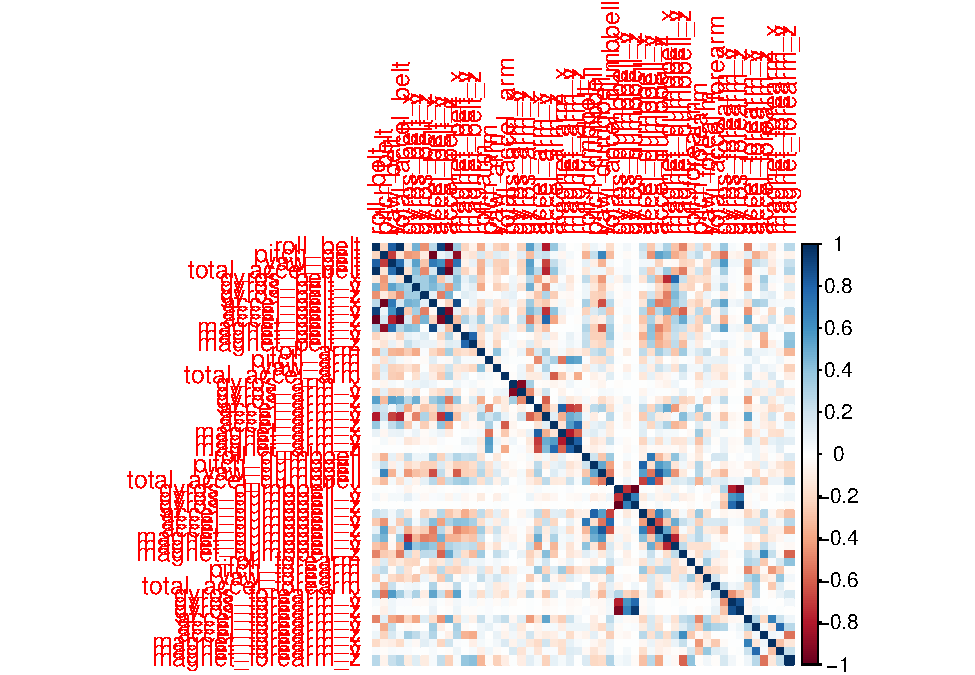
\includegraphics{pracmachlearn_files/figure-latex/unnamed-chunk-9-1.pdf}

\begin{Shaded}
\begin{Highlighting}[]
\NormalTok{treeModel <-}\StringTok{ }\KeywordTok{rpart}\NormalTok{(classe }\OperatorTok{~}\StringTok{ }\NormalTok{., }\DataTypeTok{data=}\NormalTok{trainData, }\DataTypeTok{method=}\StringTok{"class"}\NormalTok{)}
\KeywordTok{prp}\NormalTok{(treeModel) }\CommentTok{# fast plot}
\end{Highlighting}
\end{Shaded}

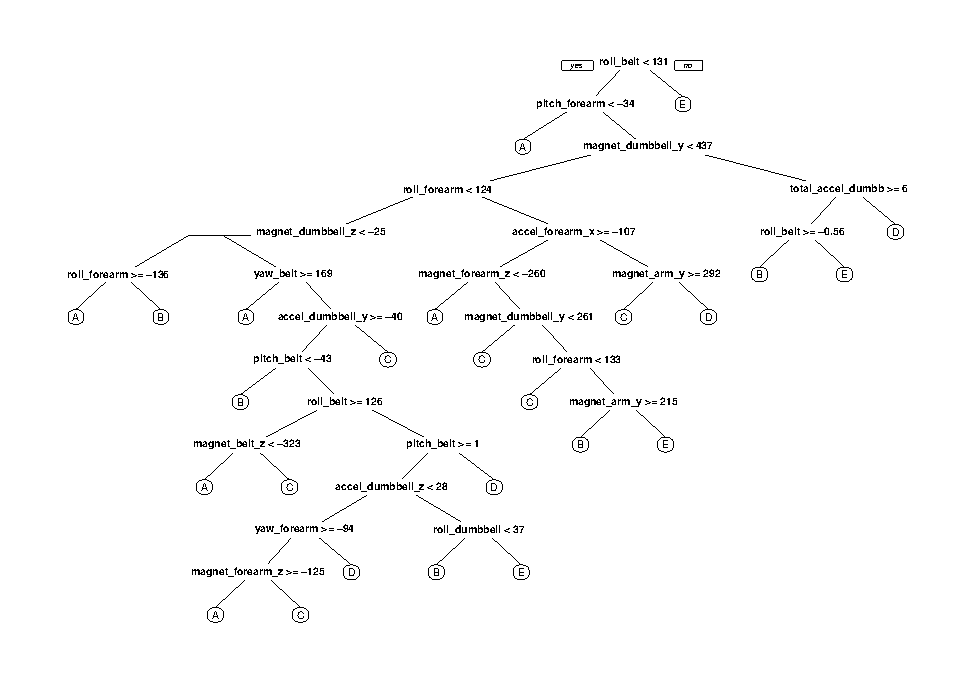
\includegraphics{pracmachlearn_files/figure-latex/unnamed-chunk-10-1.pdf}

\end{document}
